\newpage
\section{Etapa de búsqueda}
En esta etapa se realiza la búsqueda de instrucciones desde una memoria de 32 bits de ancho de palabra con 128 entradas, siendo entonces de 512 bytes. Usando el  \texttt{pc} obtiene la instrucci\'on y la saca hacia un latch para pasar a la etapa de ejecución. 

\subsection{Introducción}
La etapa de b\'usqueda de instrucci\'on tiene como entradas:
\begin{itemize}
  \item \textbf{rst}: Vuelve a todos los registros a los valores iniciales. 
  \item \textbf{enbl}: Habilita la etapa.
  \item \textbf{dec}: Entrada para la eleccion del contador del programa por si hay algun salto.
  \item \textbf{clk}: Clock de entrada a la etapa.
  \item \textbf{pc\_mux}: Bus que cuenta con el valor del contador de programa que se va a utilizar por si hay un salto.
\end{itemize} 

La etapa tiene como salidas:
\begin{itemize}
	\item \textbf{DR}: Son las instrucciones que entrega la memoria de acuerdo a la entrada que le brinda el \texttt{pc}. 
	\item \textbf{pc\_out}: Esta es la salida del \textt{pc} que se traslada a la etapa de decodificaci\'on por si hay una instrucci\'on de salto. 
\end{itemize} 

\begin{figure}[H]
\centering
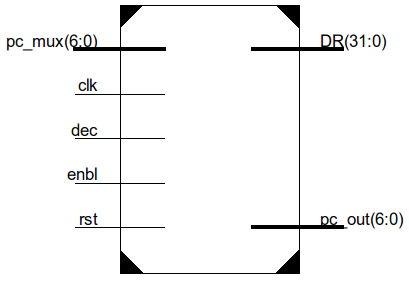
\includegraphics[scale=0.35]{Capitulo01/fetchstage}
\caption{Etapa de b\'usqueda}
\label{fig:fetch}
\end{figure}

\subsection{Funcionamiento}
El \texttt{pc} comienza de 0 y este valor entra en la memoria de instrucciones y en un m\'odulo sumador. En la memoria para que utilice la instrucci\'on ubicada en la posici\'on del mismo valor de contador de programa, y en la entrada del m\'odulo sumador se aumenta en 1 el valor para poder avanzar en el pr\'oximo ciclo de clock a una nueva instrucci\'on. Las salidas de esta etapa son la instrucci\'on a ejecutar y el valor del contador de programa.  (ver Figura \ref{fig:fetchzoom})

\begin{figure}[H]
\centering
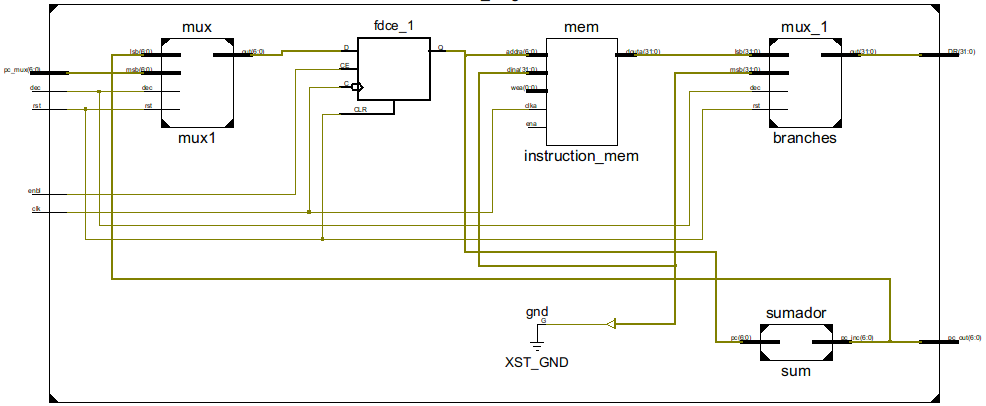
\includegraphics[scale=0.35]{Capitulo01/etapafetchzoom}
\caption{Etapa de b\'usqueda}
\label{fig:fetchzoom}
\end{figure}

\subsection{Multiplexor}

El m\'odulo multiplexor es binario, o sea que solamente elige entre dos valores. En nuestro caso debe escoger entre el \texttt{pc} que viene incrementado desde el m\'odulo sumador o el que viene modificado por un salto desde la etapa de ejecuci\'on. 

\begin{figure}[H]
\centering
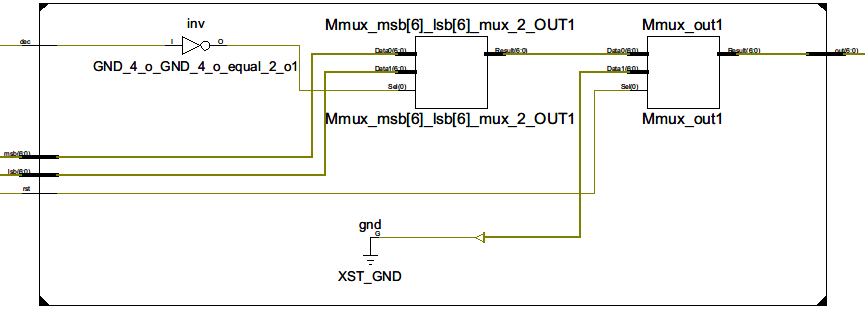
\includegraphics[scale=0.4]{Capitulo01/mux_fig.png}
\caption{M\'odulo multiplexor}
\label{fig:muxmodule}
\end{figure}

En la entrada del multiplexor entran 12 cables para que elija entre la parte alta y la parte baja, dependiendo de si es 1 o 0. Como lo programamos, cuando \texttt{dec} est\'a en uno elige el \texttt{pc}  que viene incrementado. En el otro caso, elige el que esta modificado por la etapa de ejecución.

\begin{figure}[H]
\centering
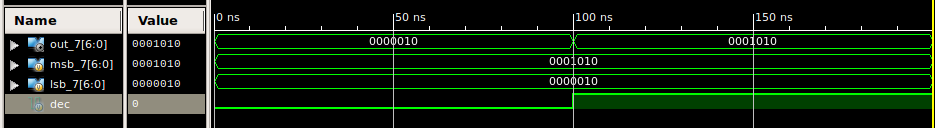
\includegraphics[scale=0.4]{Capitulo01/mux_test}
\caption{Testbench del multiplexor}
\label{fig:muxt}
\end{figure}

\subsection{Incremento}
El m\'odulo sumador simplemente incrementa el \texttt{pc}, tiene solamente una entrada que es un bus de 7 bits y este valor es incrementado dentro del m\'odulo. 


\begin{figure}[H]
\centering
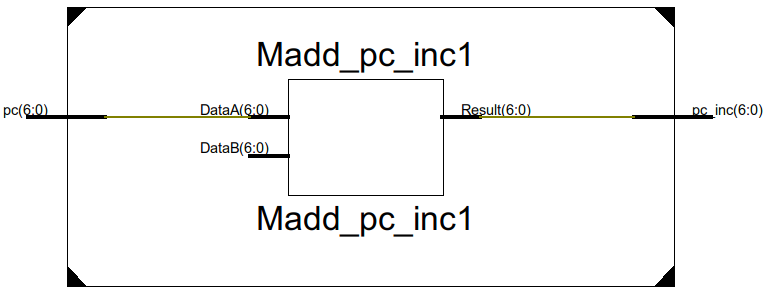
\includegraphics[scale=0.45]{img/sumador_inside}
\caption{Modulo sumador}
\label{fig:sumador}
\end{figure}


En el testbench contador de programa se va modificando de a uno, entonces la salida que en este caso es \texttt{pc\_inc} y esta ingresa en el registro del \texttt{PC}. 


\begin{figure}[H]
\centering
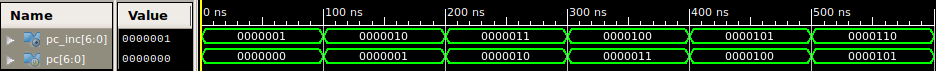
\includegraphics[scale=0.45]{Capitulo01/sum_test}
\caption{Testbench del sumador}
\label{fig:sumt}
\end{figure}


\subsection{Etapa de búsqueda con m\'odulos integrados}
Finalmente generamos un m\'odulo que integra los m\'odulos anteriores y terminamos la etapa. En este clock solamente el registro \texttt{pc} cambiaría de valor. 

\begin{figure}[H]
\centering
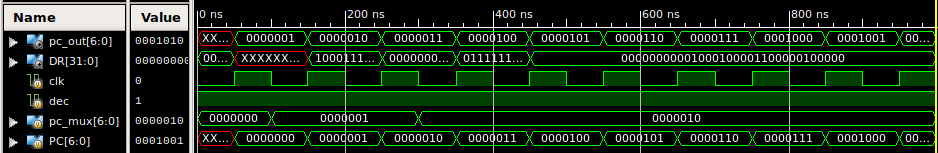
\includegraphics[scale=0.45]{Capitulo01/fetch_test}
\caption{Testbench del modulo fetch}
\label{fig:fetcht}
\end{figure}

Para entender que hace esta etapa podemos ver los cambios en la figura \ref{fig:fetcht}. Debemos comenzar viendo que \texttt{PC} no tiene ning\'un valor y es el que le ingresara en el clock a la memoria de instrucciones, \texttt{pc\_out} tampoco contiene ning\'un valor y este entra en el multiplexor (la memoria de instrucciones se puede ver en \ref{a.coe}).  
En el primer clock ascendente como \texttt{dec} esta en uno, elige \texttt{pc\_mux} para escribir al \texttt{pc} todos ceros, o sea, la primera direccion de memoria. El \texttt{dr}  muestra solo x porque en el clock anterior el \texttt{pc} estaba en x y en la memoria no direcciona en ninguna posici\'on valida. En el pr\'oximo clock ascendente ya el \texttt{pc} contiene ceros por lo que autom\'aticamente \texttt{pc\_out} va a tener el valor de \texttt{PC} + 1, pero \texttt{dec} esta en 1 por lo que sigue eligiendo a \texttt{pc\_mux}, que en el clock descendente anterior ya se le hab\'ia aumentado el valor en 1 por lo que este valor va a ser ingresado en el pr\'oximo clock al \texttt{pc} y \texttt{dr} ya comienza a mostrar el primer valor de la memoria de instrucciones. Los siguientes clocks funcionan de la misma manera.

\lstinputlisting[label=a.coe, caption=Contenido de la memoria de instrucciones, captionpos=b]{Capitulo01/a.coe}